As computer systems are used more and more for problem solving, the complexity of the systems grows just as much;
they are also becoming more dynamic due to the devices mobility, modifications in the environment of execution,
software updates, hardware upgrades, maintenance events and hardware components replacements(Salfner, Lenk and Malek 2010).
The classical reliability theory that concerns the computer systems or the conventional approaches put in place for
problem solving present a significant lack of consideration of the actual state of the computer systems as they are
not capable to offer a reflection for the dynamic and the unforeseen runtime of a computer system or the failure of
processes. These approaches are usually used in order to create a design that will allow for a long term or average
functionality predictions to solve the technical problems that occur in computer systems in an optimal and efficient
way when considering time and cost as the main factors of evaluation (Salfner, Lenk and Malek 2010). Wright-Whyte (2018)
suggests that the majority of the businesses present a specific part or sector that requires computer systems or
technological systems in order to solve the problems that the businesses are asked or required to do so in order to
speed their workflow and to ensure their existence, for this reason the computer systems are a vital component when
it comes to the ability of a business to function properly even for those businesses that are not specifically related
to information technology. Every year the failure or downtime of computer systems has led to costing businesses
around £3.6 million, a research in this area has concluded that technical problems related to computer systems can impose
costs on businesses from an average of £4,300 per hour to an even higher value which is an average of £258,000 per hour.
The downtime or the failure events related to computer systems not only affect the businesses by implying more costs in
order to solve the technical problems, but also affect the staff working for those businesses, as approximative 545 hours
of staff activity are lost every year because of computer systems failure or downtime events, for specific countries like
the United Kingdom where the staff average wage it is more than £13.75 per hour, this will lead to an average of £7,235 that
a business will have to pay for one employee only every year in order to rectify or provide assistance for the technical
problems of the computer systems that have presented some runtime failure or the downtime event during their assigned
sessions, the failure or downtime event also permitting a decrease in the normal functionality of the business or even
worst, stopping the business to have any relevance at all (Wright-Whyte 2018).
\newpage
The failure or downtime of computer systems it is an event that can be categorised as virtually inevitable, at some point in time the failure or downtime will occur
and the businesses that make use of computer systems or technological systems will be affected by it, the frequency and
duration of the failure or downtime event will vary as this is dictated by the technical problems, but the businesses
will have to suffer the costs despite the reason of computers failure, business size or the success of the business.
The failure or downtime of computer systems can be defined as an occasional period of time when a computer system or
an essential part of a technological system it is no longer functional or it cannot be used at that point time, the
result of computer systems failure or downtime will impose a cost on any business that makes use computer systems for
problem solving and this cost will be detrimental.
The computer systems failure or downtime will occur due to human error, power outage, unreliable equipment, hardware or
software failure. The failure of computer systems can have a negative effect on the businesses that will be put in the
situation of solving this kind of problems by not only stopping the normal functionality at the moment of failure or
downtime of the business but also creating long term consequences due to this event (Wright-Whyte 2018).
The instant effect or the short term effect of the computer systems failure or downtime will not present any financial
problem that can be felt at the moment of computers systems failure or downtime, but the negative aspect of the failure
or downtime event can be represented by the productivity time being lost due to this event and this will lead to a
decrease in the profit made by the business. Other short-term effects of computer systems failure or downtime are the
loss of productivity, labour and cost investment into investigating and solving the technical problems and the fact
that the business will not be able to function in normal parameters. The long term effects caused by the computer
systems failure or downtime cannot be ignored as they will have a significant impact on any business that will face
the computer systems downtime event, the most important long term effect caused by a potential computer system
failure or downtime it is the negative financial impact on the business, the impact will initially seem like
short term effect but it could lead to a more significant loss of profit in the long run if the problem is not solved
in short period of time. Beside the financial impact on the business caused by the failure of the computer systems
or the downtime event are the decrease of employee’s morale within the business and the business image and reputation
which can be considered also as long terms effects due to the downtime event (Wright-Whyte 2018).
In May 2017, the failure of computer systems or downtime event caused by a power outage in data centre situated in the
west of London lead to the unavailability of the British Airways systems in 70 countries resulting in the inability of
the British Airways staff to check-in passengers, this was a relatively short time event as it lasted only 15 minutes,
but it can be easily seen what impact it can have on a business as thousands of flights were cancelled with an estimated
75,000 customers being affected by this computer systems failure or downtime event (Wright-Whyte 2018).
The implications of computer systems failure or downtime event must be known by any business despite of business size
or success as planning in advance for such events and being able to take actions for them that could mitigate or even
eliminating the impact of a possible downtime events will give some advantages to the business in cause comparing to
the competitors (Wright-Whyte 2018).
\newpage
The focus of this research is to try to forecast possible events that could lead to computer systems failure by
reviewing and then selecting the right computer systems failure predictions methods when hardware sensors are an
important element for the predictions that will allow the limitation of the impact of such failure events by
allowing the right measures to be put in place before this kind of events will occur by providing a time interval
where actions can be taken.

\
\begin{figure}[h]
    \centering
    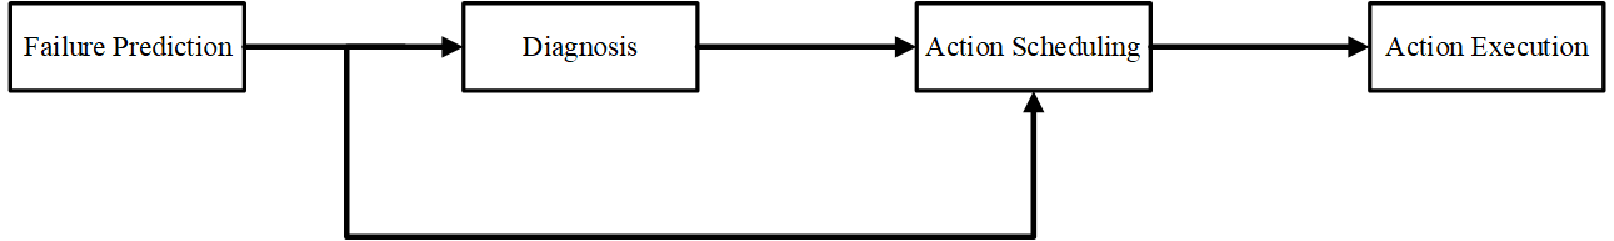
\includegraphics[width=1.0\textwidth]{images/failure_steps.pdf}
    \captionsetup{justification=centering}
    \caption[Workflow support for failure management]{Workflow support for failure management
                                                     (Salfner, Lenk and Malek 2010 p. 3 fig. 2)}
    \label{fig:failure-steps}
\end{figure}

The Figure 1 shows the steps involved in failure management, once a failure event has been predicted,
the prediction should be accompanied with a diagnosis in order to find out the root of the problem
that will cause further upcoming failure events, the role of the diagnosis is to allow the selection
of the right decision when it comes solving the problem using the right method and scheduling the
execution of the task (Salfner, Lenk and Malek 2010).

\section{Root Causes, Faults, Errors and Failures}

According to Wu and Buyya (2015), there is a lot of statistical research that shows the relevance of the human factor
in both planned and unplanned downtime, as it can be seen in the Figure 2, it is a reasonable root cause for the
computer systems failure or downtime, for the unplanned downtime the human error factor represents 15\%
of all unplanned downtime and for the planned downtime which represents 30\% of all downtime events in data
centres there is also a certain percentage of human error that will trigger the computer systems failures,
if the planned downtime would be eliminated, then the percentage of human error factor will increase to a value
of 18\% (see Figure 3). As it can be seen in the figure 2, the majority of faults or failures are caused in
large part by the software element, comparing to the hardware element, but nevertheless, the hardware element
representing 10\% of all computer systems failures or downtime events cannot be overlooked as this number it
will have a significant impact of the runtime of computer systems if failure predictions are provided based
on the hardware element.

\newpage

\begin{figure}[h]
    \centering
    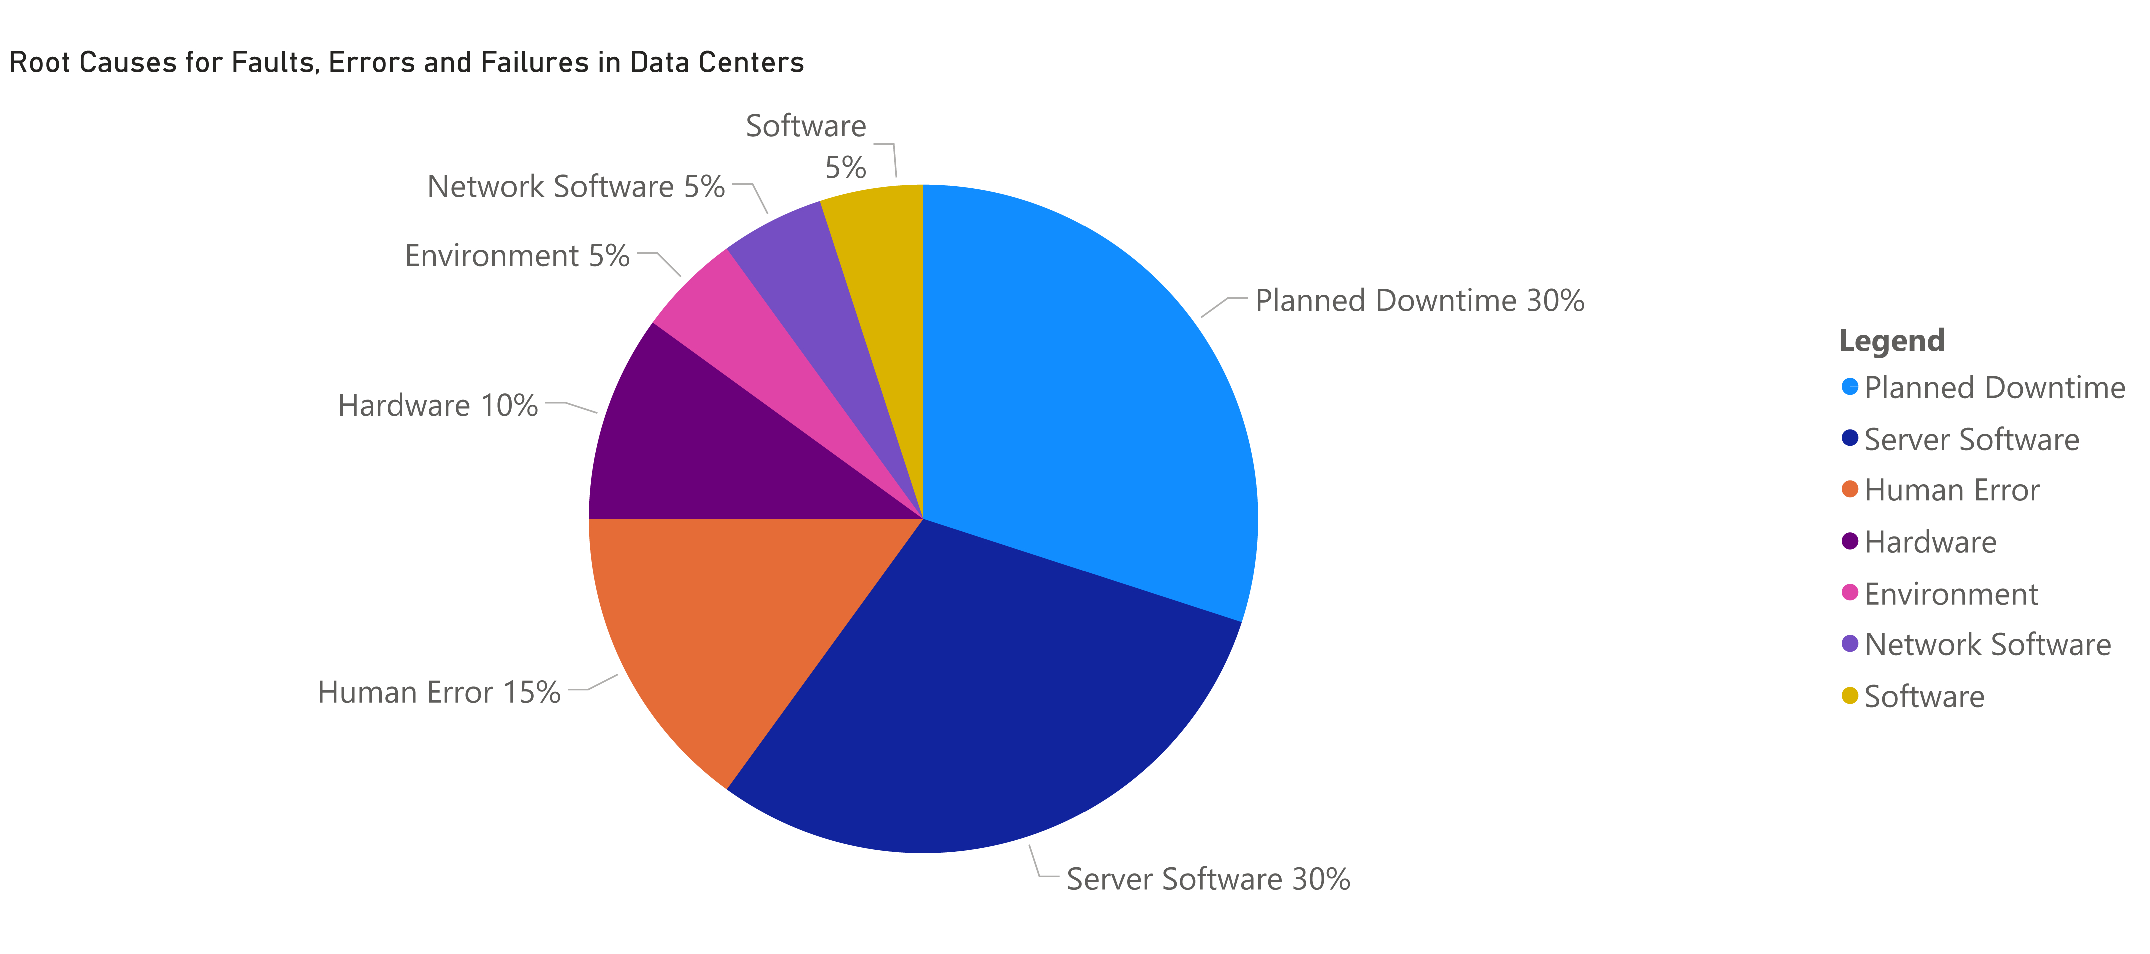
\includegraphics[width=\textwidth]{images/downtime.pdf}
    \captionsetup{justification=centering}
    \caption[Errors, faults and failures in data centres]{Errors, faults and failures in data centres
    (Wu and Buyya 2015 p. 360 fig. 10.8)}
    \label{fig:downtime-events}
\end{figure}

In critical applications, the human error play an important role when talking about computer systems failure or
downtime events, as the human error increases to a more substantial level for critical applications, this
substantial level has the potential to reach a value of 40\% from the operation errors and system outages,
these two elements making 55\% and respectively 22\% of all critical applications failure events or downtime
events (Wu and Buyya 2015). The human error factor represents a significant value of 18\% of all computer systems
failure or downtime events in data centres, Wu and Buyya (2015) suggest that the reason for this substantial value
of human error it is caused by the changes represented by the software upgrades, software patches, system
reconfigurations and maintenance events scheduled for the data centres. These fundamental elements cannot be
banned for a computer system or even more important for a data centre for security reasons and also because
changes are inevitable, an insight into other elements must be performed in order to provide solutions to the
computer systems failure problem, these elements being the hardware element and the networking transmission element,
they are not as predispose to changes as the other mentioned elements and because of this they are good candidates
for computer systems failure predictions.

\begin{figure}[h]
    \centering
    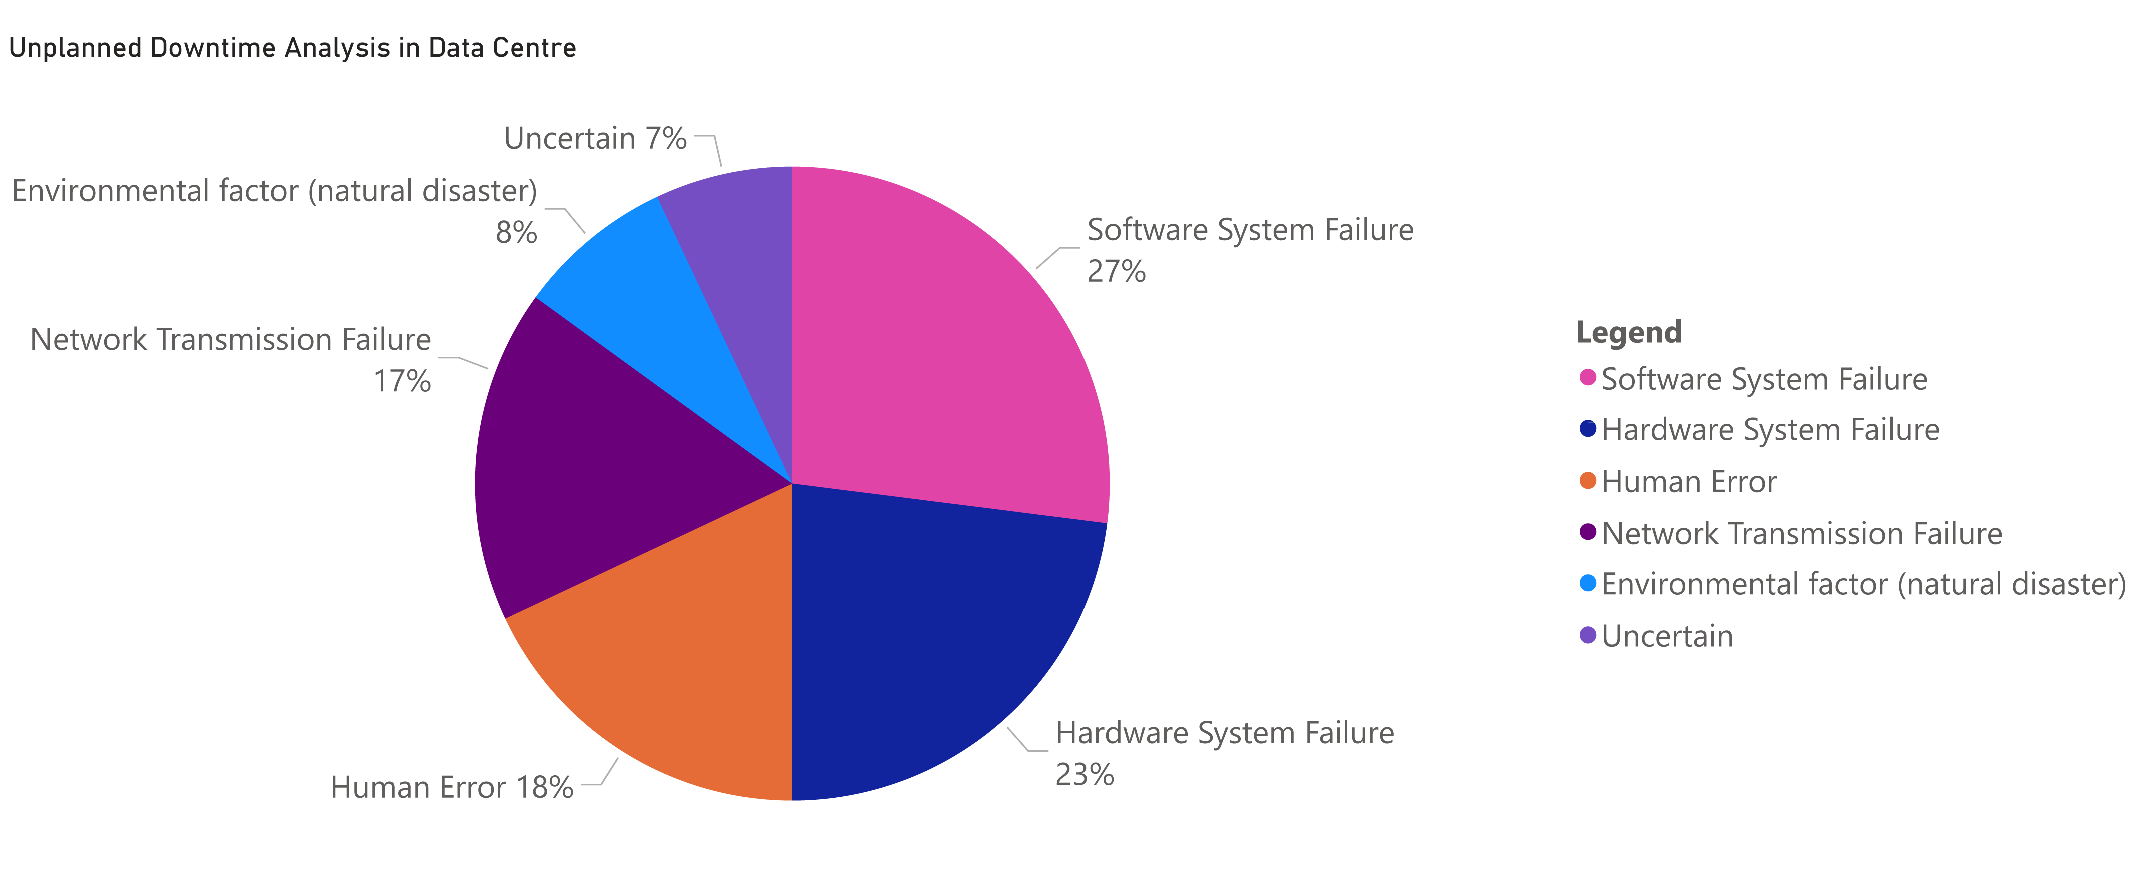
\includegraphics[width=\textwidth]{images/unplanned-downtime.pdf}
    \captionsetup{justification=centering}
    \caption[Unplanned downtime in data centres]{Unplanned downtime in data centres
    (Wu and Buyya 2015 p. 361 fig. 10.9)}
    \label{fig:unplanned-downtime}
\end{figure}

\begin{figure}[h]
    \centering
    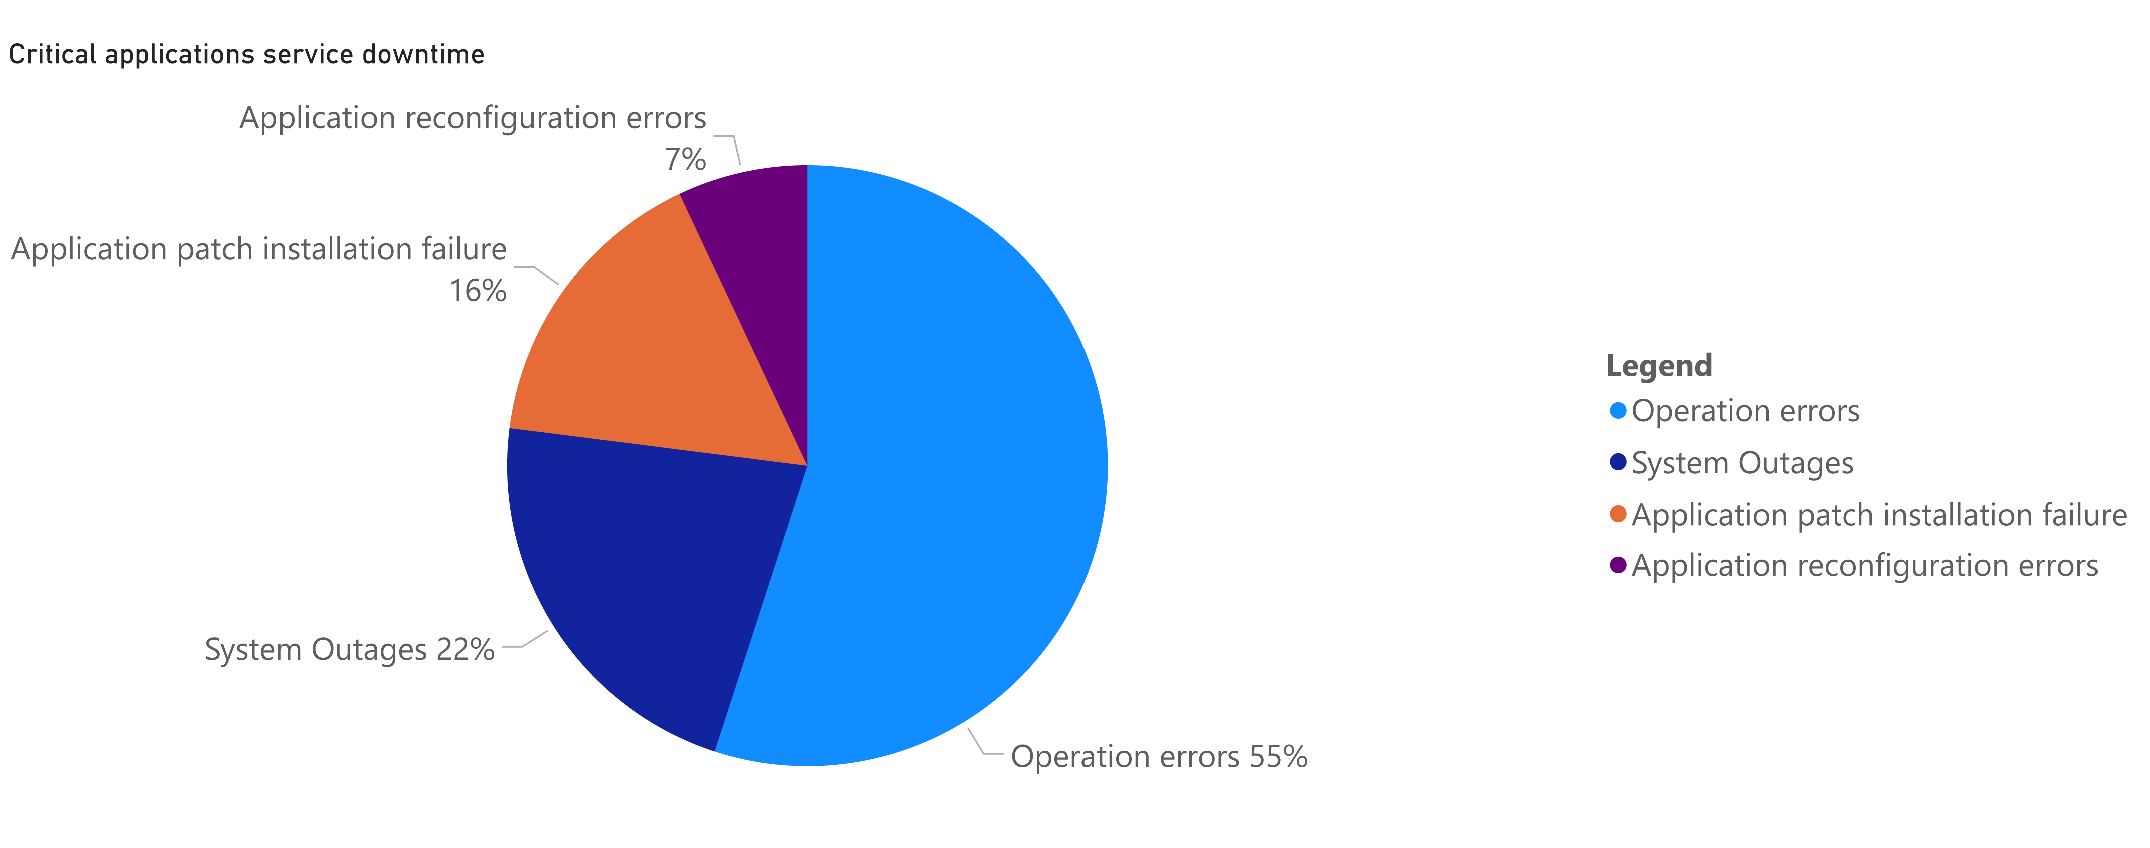
\includegraphics[width=\textwidth]{images/critical-applications-service-downtime.pdf}
    \captionsetup{justification=centering}
    \caption[Critical applications service downtime]{Critical applications service downtime
    (Wu and Buyya 2015 p. 361 fig. 10.10)}
    \label{fig:critical-applications}
\end{figure}

\clearpage

\section{Opportunities and Motivations}

The computing elements and their general influence over data centres mentioned in the Root causes, Faults, Errors and
Failures section naturally bring into discussion the term “Maintenance of Computer Systems”, as this term becomes
relevant for enterprises, institutions, organisations and individuals that need to monitor the performance and state
of their computer systems in order to prevent, mitigate and evaluate the impact of events such as slow response of
the computer systems, the computer systems not responding when specific operations are performed or worst the
failure of the systems which would result in the transition of the system from a working state to a non-working
state accompanied with the loss of essential data. According to Baldoni, Montanari and Rizzuto (2014) a few years
ago the use of proprietary systems provided by a single vendor was a convenient and preferred approach for specific
safety-critical systems related to sectors such as air traffic control, railway control, commercial aircraft and
nuclear power. In addition to those said before by Baldoni, Montanari and Rizzuto (2014), according to Sipos, Moerchen,
Fradkin and Wang (2014) failure predictions can also be used in medical institutions where the medical equipment
it is the core element in the failure predictions process, the logs provided from the medical equipment are
retrieved and used in the maintenance prediction process. Beside the use cases mentioned above, the individuals
that may be concerned about the computer systems failure predictions or downtime events predictions would be
professionals working as computer technicians or systems administrators which are usually assigned with tasks of
ensuring the normal functionality of specific computer systems it is present. The professionals working as
technicians or system administrators would benefit the most from this type of desktop application, as the time
invested into the investigation of hardware or software technical problems could be reduced or even eliminated
by providing near real-time information about the state of one or more monitored computer systems and the
prevention of events that may require maintenance such as the failure of the computer systems which could
vary from the event of a non-responding machine to the transition of the machine from a working state to a
non-working state could be possible if a prediction of hardware or software technical problems is provided
based on past data collected from the computer systems. As it was mentioned before in the Root causes,
faults errors and failure section it is safe to say that data centres, medical institutions, air traffic
controls, railways controls and power plants will benefit the most from computer systems failure predictions
because these kind of predictions will allow the minimization of computer systems failure impact on each of
the entities mentioned if the right measures are put in place before it happens. The applications, services
and resources of a desktop or even server type of computer systems could be organized and scheduled in
a manner which would reduce the impact of the system’s failure whenever predicted by making use of right
techniques which would fit the equipment in cause and classify specific events that would occur in computer
systems as events that would require maintenance or just as informative events if the severity of the events
is low in order to secure the normal functionality of the machines.

\section{Maintenance Solutions}

According to Bastos, Lopes and Pires (2014) in an industrial environment where equipment availability it is
a vital factor in order to ensure the productivity of organisations, the maintenance activities are performed
in order to reduce or eliminate the failures of specific equipment or machinery and with this creating
favourable conditions and allow an increase of productivity for the business or organisation in cause.
The satisfaction of businesses or organisations usually implies the increase of pressure in maintenance systems,
the maintenance process even being considered not to add any value to the businesses or organisations,
but nevertheless the maintenance process it is an important factor that will contribute to the reduction of
business or organisation costs and allowing the equipment to function in normal conditions. The main factor
of acknowledgment related to computer systems or technological systems failure are some indicators that will
proceed such failure events in 99\% of the maintenance events cases. The breakdown maintenance or runtime
failure also called as the unplanned maintenance event it is the earliest maintenance technique which takes
place at the breakdown event of the machine in cause, the later technique it is a preventive technique which
will allow a time interval to take actions also called as planned maintenance (Bastos, Lopes and Pires 2014).
The problem of maintenance of computer systems or technological systems presents both commercial and open
source solutions, these solutions can be categorised as reactive maintenance solutions and predictive
maintenance solutions. The reactive maintenance solutions can be defined as a mechanism that can be used to
respond to technical problems that have occurred in computer systems or technological systems at a specific
point in time where no time interval has been provided by the solution in cause in order to take any measures
that could be used to mitigate the impact of the technical problems that have occurred in the system in cause,
it is safe to say that a reactive maintenance solution will allow a response to the maintenance events after
the impact has been felt by the computer system or technological system in cause. The predictive maintenance
solutions can be defined as a mechanism that will allow the provision of an informative event related to a
possible technical problem that is likely to occur in the near future in a computer system or technological
system accompanied with a diagnostic that will contain the root cause of the technical problem and time
interval where actions can be performed in order to mitigate the impact of the maintenance problem
(Bastos, Lopes and Pires 2014).

\newpage

\section{Challenges and Impediments}

According to Salfner, Lenk and Malek (2010) the core elements that contribute to the challenges and impediments
of computer systems failure or downtime events are the dependability and resilience factors. These factors are
represented by the continuous increasing of computer systems complexity, the continuous increasing of cyber
security problems such as attacks and threats, the continuous increase of connectivity and interoperability
of technological systems, the increasing use of third party and open source software and last but not the
least the dynamic and unforeseen runtime of computer systems. The dynamicity of computer systems can be
reflected by the frequent system configurations, system reconfigurations, software updates and hardware upgrades.
The elements that contribute to the difficulty of computer systems failure predictions mentioned by Salfner, Lenk
and Malek (2010) are not the only factors that will increase the difficulty of failure predictions when talking
about computer systems or any technological systems. In order to provide maintenance predictions signals for a
technological system, an insight must be taken into the running state of the technological system or equipment
in cause, this insight it is performed either by making use of the existing hardware sensors present on the
components of the technological system or the equipment in cause or additional hardware sensors will be added
to the technological system’s components or equipment in order to allow the recording and retrieving information
such as temperature signals, voltage and other information of interest, once the hardware sensors have been put
in place or they already exist on the technological system or equipment, the failure or maintenance predictions
module can then send alerts or signals of possible events that will inform the control centre of any components
values deviating from normal parameters, these deviations of values are an important factor in predictive
maintenance as this deviations of values could result in the failure of the technological system or equipment
in cause (Sipos, Moerchen, Fradkin and Wang 2014). A more technical approach and confirming the continuous
increasing of computer systems mentioned above  there are other elements that will increase the difficulty of
computer systems failure predictions, according to Botezatu, Giurgiu, Bogojeska and Wiesmann (2016) when
adventuring into computer system failure predictions a known fact is that all computer systems will present
a storage system, this system being an important component and also the root cause of the most computer system
failures in data centres, in most cases this storage system it is a hard disk and usually all hard disks present
a mechanism called Self-Monitoring, Analysis and Reporting Technology (S.M.A.R.T), this mechanism will contribute
to the difficulty of trying to predict unforeseen failure events based on the storage system. The dynamicity of
the hard-disk S.M.A.R.T indicators will be the main factor of difficulty as these indicators are manufacturer
specific, the specialised encoding of the hard disk indicators will be different for each hard-disk model and
their normalization values will also vary depending on the manufacturers.

\newpage

\section{Hardware Sensors}

The hardware sensors in computer systems or technological systems have the role to measure the physical behaviour
of specific components that the machines or technological systems present in their composition, these computer
systems or technological systems usually are executing cyber space but this is not a requirement for the hardware
sensors in order to be present on the components of the computer systems or technological systems in cause.
In addition to the physical behaviour measuring or monitoring of the components, the hardware sensors also
sample the physical effects of the processes that allow the transfer and processing of information.
The hardware sensors can monitor or measure the behaviour of computer systems components from the internal
input and output channels to the LED status of the lights and for this reason the hardware sensors are an
important element when trying to make predictions related to computer systems failures or downtime events
(Edgar and Manz 2017).

\subsection{Processor}

The \acrfull{cpu} sometimes referred as the Central Processor or simply just as Processor it is
a hardware component which can be considered the brain of a computer system, this component it is considered
the brain of a computer system because it is the place where the most calculations take place in a computer system.
The Processor has the role to execute the instructions of a computer program which are retrieved from the memory
of the computer system in cause and because of this in terms of computing power it can be considered the most
important piece of hardware in a computer system (Beal 2020). According to Bach (2014) it is a known fact that
modern computer systems processors present some mechanism of active cooling in order to ensure their normal
functionality without producing a runtime failure but there is a little official information on how the modern
processors are affected by different temperatures when it comes to their performance. When it comes to older
computer systems processors the behaviour presented by this chips when encountering high temperatures would be
a failure of \acrfull{cpu} which will result in the transition of the working machine to a
non-working machine caused by the overheat of the processor component, the modern computer systems on the other
hand have the capability to adjust their frequency according to the temperature they are functioning at in order
to prevent the failure of the technological system in cause, this prevention of failure has the drawback of a
decrease in the performance for the processor in cause as the temperature increases the processor will try to
protect itself and slowing performance (Bach 2014). The \acrfull{cpus} or Processors are not excluded
from the zone of possible failure, the processors can fail if the conditions of failure are present but most
processors are one of the most reliable components in a technological system or workstations as \acrfull{cpus}
have a small overall failure rate of just 0.2\%, this will result in a single processor failing in
500 of processors when the components are of production process and delivered to the customers (Bach 2014).
It is safe to say that using the temperature sensors of the processor component will not present a good candidate
for failure predictions but it may present a good candidate for anomaly detection.

\newpage

\subsection{Memory}

The computer systems memory it is a term used to represent multiple types of data storage technologies that computer
systems can use, these types of memories are the \acrfull{ram}, the \acrfull{rom} and Flash
Memory (Rubens 2019). The computer systems present many types of memory, the most common distinction is between
primary memory and secondary memory, the latter one being more commonly known as storage memory. The primary
memory includes the \acrfull{rom} and \acrfull{ram} and it is located close to the \acrfull{cpu} or
Processor on the computer motherboard, allowing the Processor to read data from the
primary memory in a relatively fast manner, in other words the primary memory has the role to store data that
the \acrfull{cpu} will need to have access as soon as possible and not being required to wait
for delivery of data. The secondary memory most commonly it is usually physically located in a separate storage
device, for example a \acrfull{hdd} or a \acrfull{ssd}, the secondary memory in cause being
connected to the computer system in a direct way via a \acrfull{sata} cable or
over a network (Rubens 2019). The \acrfull{ram} as the name implies it has the role to store data
that can be accessed in a random manner, this type of memory it is fast to read and write which makes it a
volatile type of memory. The Read-Only Memory as the name implies it has role to allow data to be read from
this type of memory and no data can normally be written to it. According to Bach (2019)  the \acrfull{ram}
used to be one of the most reliable pieces of hardware but in the last 5 years it has improved
even more, the \acrfull{ram} has an overall failure rate of 0.41\%, this value will result in a
single Random Access Memory will fail out of 244 of \acrfull{ram} hardware components, but the
failure rate presented on the customers side or the field failure rate had a value of 0.07\%, this value
representing a single failure out of 1400 of \acrfull{ram} sticks once the components are
presented in the customers possession. It is safe to say that using the sensors of the \acrfull{ram}
component will not present a good candidate for failure predictions but it may present a good candidate
for anomaly detection when considering the voltage as the main factor of analysis.

\newpage

\subsection{Storage System}

Data storage can be represented by the collective methods and technologies that allow the capture and retainment
of digital information on entities such as electromagnetic, silicon and optical storage media. The word storage
is used most of the time to represent the devices connect to a computer system, the connection being made through
input and output operations, these includes Hard-Disks, flash media and other media entities. These days the main
types of storage media are the Hard-Disk Drives, Solid-State Drives and optical storage, the Hard-Disk
Drives are widely used to store data in computer systems used as personal computer, servers and enterprise storage
systems but the Solid-State Drives are also start to present an increase in the use for similar purposes (Rouse 2018).
According to Botezatu, Giurgiu, Bogojeska and Wiesmann (2016) the costs caused by computer systems failures or
downtime events have increased in a significant way in the past years for data centres, these costs are ranging
from the minimum cost of \$5,600 per minute in 2010 to the maximum cost of \$8,851 per minute in 2016. The failure
of technological equipment it is the most important factor that contributes to the downtime events. The Hard-Disks
Drives are one of the most frequent components to fail in a computer system or in information technology environments.
The reliability and performance of the Hard-Disk Drives are affected especially by factors such as duty cycles,
workloads and temperature, the reliability problems are the most important as the severity of these problems will
cause the failures of the hard-disk drives and eventually the need to replace the hard-disks in cause. Hard-Disk
Drives failures can be categorised as either predictable failures or unpredictable failures, the unpredictable
failures are represented mostly by the electronic components of the hard-disk in cause not being functional anymore,
this event being sudden without any warning of possible crashes and because of this the unpredictable failures
caused by the electronic components cannot be predicted by monitoring. The predictable failures on the other hand can
result from slow processes represented by normal usage of the component that usually progresses over time, most of
the time over month or years. The latter one will allow the analysis of possible predictive failures. The hard-disk
drive sensors or the \acrfull{smart} system can be used to monitor the
factors that will cause the failure of the hard-disk or when a failure is most likely to occur. Most of the time
manufacturers implement a system that makes use of these S.M.A.R.T attributes in order to provide predictions of
possible failures for the hard-disks, but these embedded models are not very efficient as they present minimal
considerations of the technical problems that could occur and for this reason are considered simple models that
cannot offer an insight about the unforeseen failure events due to the threshold-based normalisation, the focus of
the design being on avoiding false alarms of possible failures. According to Klein (2020) Blackblaze was in the
possession of 150,757 hard drives used to store customers data, as of 30 September 2020 an evaluation of the
reliability of these hard-disks was performed, this evaluation resulted in an overall or annual failure rate
of 0.89\% for all hard-disk drives. It is safe to say that using the sensors of the Hard-Disk Drives
component or the S.M.A.R.T indicators will present a good candidate for failure predictions as it is a component
that is frequently causing computer systems or technological systems to fail and it has the necessary attributes
in order to make the predictive alerts happen.

\section{Software Implications}

The manufacturing companies depend generally on the reliability of the products that are being produced by the
companies in cause in order to have success and to ensure their existence. This dependability that the manufacturing
companies present for the reliability of products in cause brings into discussion the scheduled maintenance of
equipment that companies are using, this scheduled maintenance it is a necessity for this kind of companies in
order to ensure the normal functionality and the avoidance of possible failures of any kind of technological
systems or equipment, the scheduled maintenance in this case it is used as a safeguard. The maintenance it is
performed separately most of the time for all components, the selection being made on usage, performance or
simply because of fixed scheduled maintenance, just like any other activity performed within a manufacturing
company and not only, the scheduled maintenance are not free of cost, the scheduled maintenance it is labour
intensive, not free of cost and not efficient when it comes to identifying technical problems that develop
between technicians visits. Unpredictable failures of computer systems or technological systems will still
occur despite technicians’ visits, on the other hand, the predictable failures or prediction of maintenance
events related to computer systems or technological systems can determine the condition of the system in cause
and allow the repair or the evaluation that must be performed. The ultimate goal of the predictive maintenance
or the predictive failure for the technological systems in cause is to allow pro-active scheduling and corrective
activities that will result in solving the problems created by unexpected failure of the systems in cause. Modern
technological systems or information technology equipment is most of the time operated with the help of software
applications, for example in the case of medical equipment, most operations such as warnings related to scan
performed on a patient can be retrieved and used to created medical reports and to perform specific calibrations,
these activities are controlled by a software application. The software applications most of the time are producing
some king of logs to represent their operations, these logs are exist in order to inform the user of the software
application about the activities that are being performed at a specific point in time by the application in cause
or to reflect the software developers instructions or ideas about what valuable information must be mentioned, for
example error messages, internal states or exceptions. The information found in the logs provided by the software
applications can be used to trace back how a piece of hardware was used and to have an insight about the functionality
of the component in cause by analysing the content of the logs for any errors or internal state abnormalities. However,
the use of information related to technological systems or equipment found in log files can present many challenges and
impediments when it comes to failure predictions as it has not yet been fully explored and understood since logs of
software applications are used for debugging purposes they contain minimal information that can be used for failure
predictions when it  comes to technological systems or equipment, beside the minimal information the logs files also
need data pre-processing actions as the logs contain symbols, categorial variables, times series and characters which
are not structured, the data also being considerably large which will lead to time consuming analysis due to the
calculation power required (Sipos, Moerchen, Fradkin and Wang 2014).

\section{Computer Network Architectures}

Having Access to networks or to the internet especially is becoming a fundamental element and most of the time a
requirement for software applications as applications frequently need some kind of internet access in order to
provide services to the users. The \acrfull{iot} allows more and more devices to be interconnected and
because of this understanding how to have access to networks becomes a crucial element (Reese 2015).
The term Computer Network Architecture refers to the physical and logical design of computing elements such as
hardware, software, network protocols and media when it comes to transmission or transfer of data, in other words
this term can be defined as a method that represents how computers are organised and how tasks are allocated to
the computers. (JavaTPoint 2018). A computer network it is composed of nodes and links which are combined in order
to create a network architecture. A device connected to the \acrfull{iot} it is usually called a node
and a computer node is usually called host, the communications between these nodes are done by making use of
protocols such as HTTP, TCP and UDP. The network nodes can include devices such as \acrfull{nic},
bridges, switches, routers and hubs, these elements are all involved in the transmission of data between computer
systems and other interconnected technological systems. The network links can be represented by the wires such as
coaxial cables, twisted pairs, fibre optics and wireless such as Wi-Fi or satellite communications, these links
can support a range of bandwidth and address specific communication needs. (Reese 2015). The communication between
the network nodes it is done by sending a message across the internet from a home computer or any computer system,
once this event happens, the computer’s unique address is not globally unique and for this reason any messages sent
between the network nodes or the computer systems will by handled by the \acrfull{nat} device
which will allow the changes of the address to an address that can be used for the \acrfull{iot} or
simply the Internet and allow a single IP address to be used for multiple nodes on the network. There are two
types of computer network architectures, these are the \acrfull{p2p} architecture and the \acrfull{cs}
architecture (JavaTPoint 2018).

\begin{figure}[h]
    \centering
    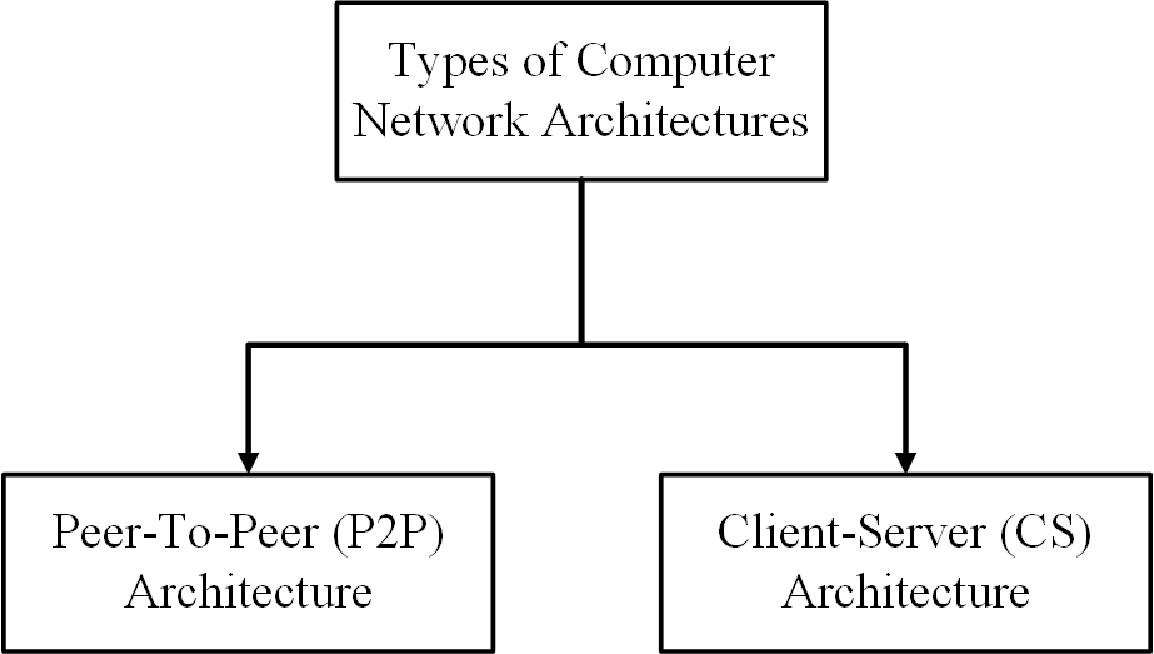
\includegraphics[width=0.65\textwidth]{images/network-architectures.pdf}
    \captionsetup{justification=centering}
    \caption[Computer Network Architectures]{Computer Network Architectures (JavaTPoint 2018 fig. 1)}
    \label{fig:network-architectures}
\end{figure}

\subsection{Data Transfer using Peer-to-Peer Architecture}

The Peer-To-Peer (P2P) network can be defined as a network where all the nodes or computer systems are linked
together and all nodes are both clients and servers at the same time with equal privileges and responsibilities
when it comes to the transfer and the process of data (Neagu 2019).

\begin{figure}[h]
    \centering
    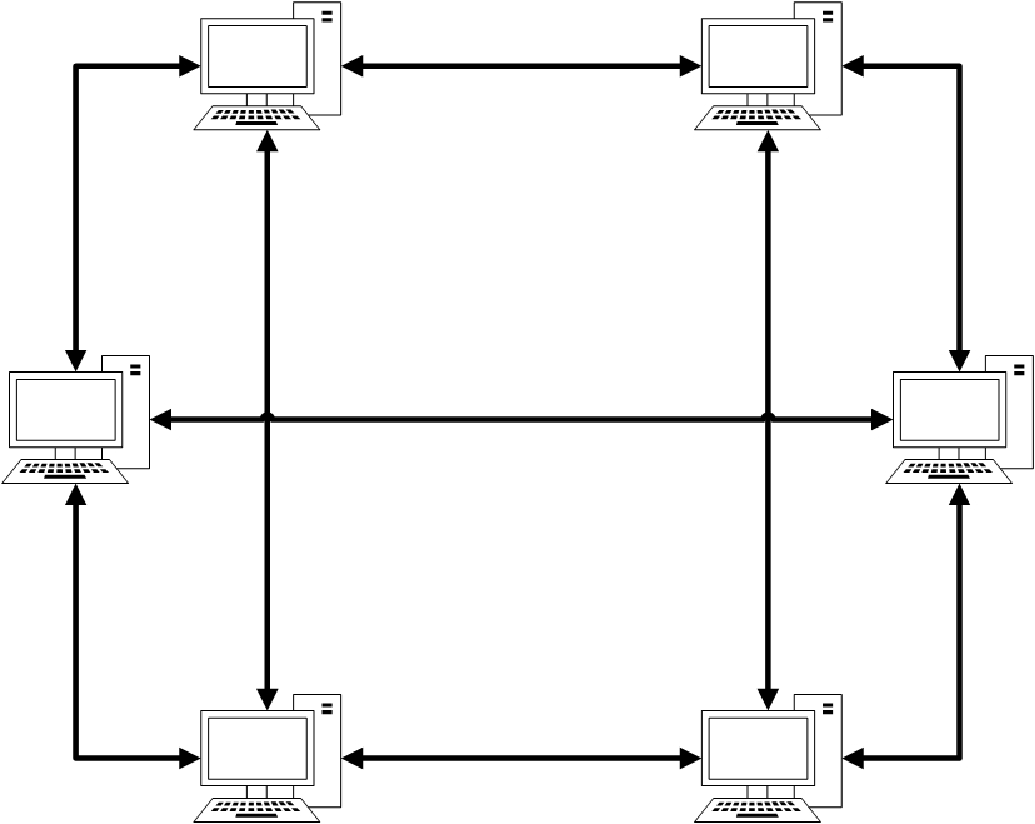
\includegraphics[width=0.55\textwidth]{images/peer-to-peer.pdf}
    \captionsetup{justification=centering}
    \caption[Computer Systems Peer-To-Peer (P2P) Simulation]{Computer Systems Peer-To-Peer (P2P)
                                                             Simulation (Neagu 2019 fig. 1)}
    \label{fig:network-peer-to-peer}
\end{figure}

\subsection{Data Transfer using Client-Server Architecture}

The Client-Server (CS) network can be defined as a network where the nodes or computer systems are linked together
to a centralised system called server, the nodes can be called clients which can access resources from the
centralised system or server as the privileges and responsibilities when it comes to the transfer and the
process of data are not equal, the server having more privileges and responsibilities (JavaTPoint 2018).

\begin{figure}[h]
    \centering
    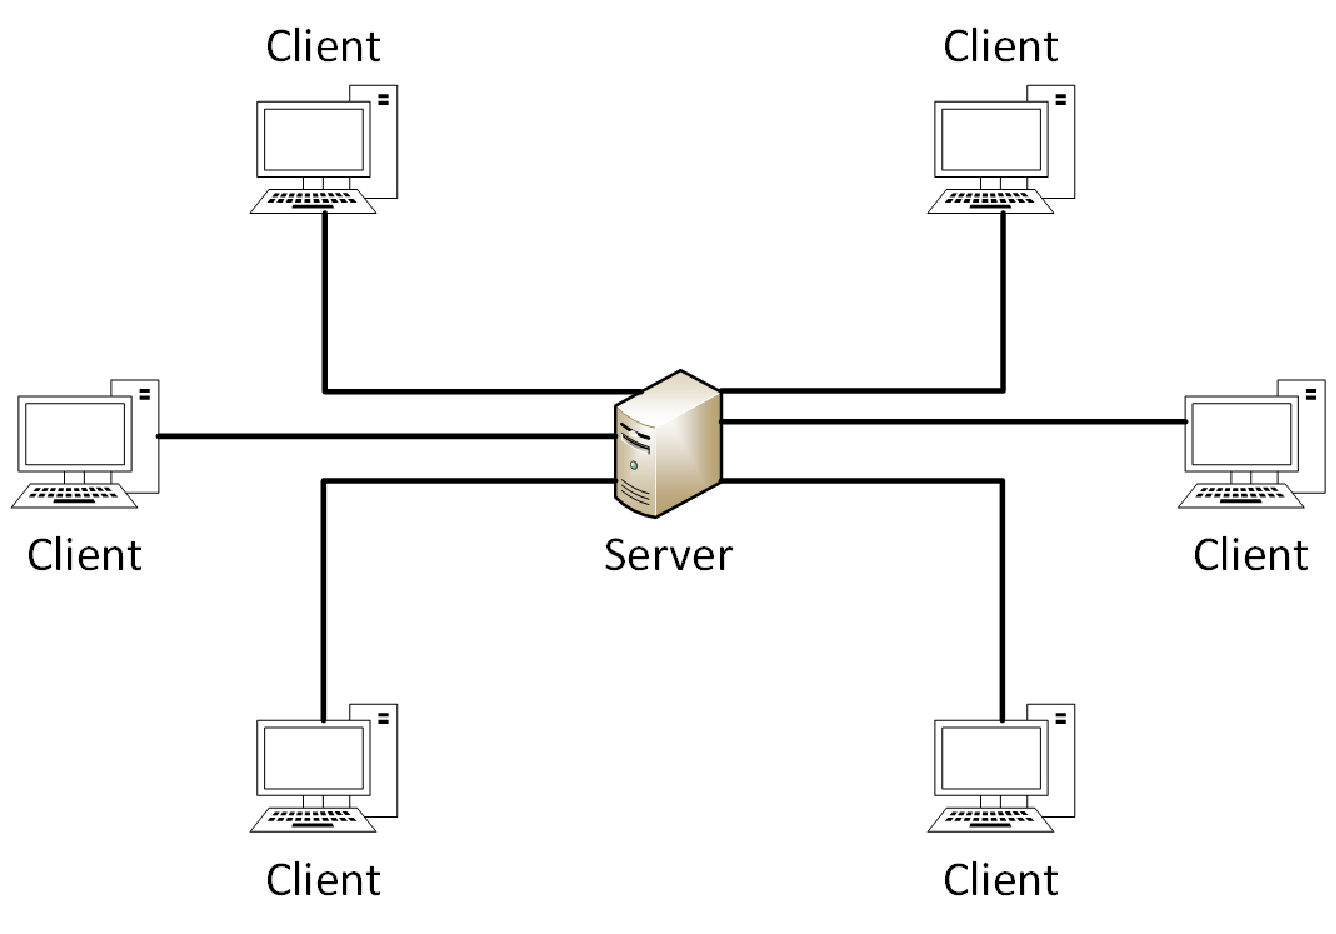
\includegraphics[width=0.55\textwidth]{images/client-server.pdf}
    \captionsetup{justification=centering}
    \caption[Computer Systems Client-Server (CS) Simulation]{Computer Systems Client-Server (CS) Simulation
                                                             (JavaTPoint 2018 fig. 2)}
    \label{fig:network-client-server}
\end{figure}

\section{Approaches and Techniques}

Numerous approaches have been performed in order to provide a solution to the maintenance of computer systems problem.
Some of the most common approaches would be the ones that make use of machine learning techniques such as
classification and regression models in order to analyse system log files which could contain data from simple
system log in information to more relevant information when it comes to maintaining a machine such as software
failure or hardware failure.  Fulp, Fink and Haack (2008) suggest that the prediction models that have been used
for the maintenance or failure of computer systems problem would be some of the standard machine learning models
such as the Bayes Networks Model, the Hidden Markov Model and Partially Observable Markov Decision Process,
these models have been used in association with an analysis of operating systems events logged and stored on
the computer’s hard-disk in order to be able to signal any occurring failure of the system in near real-time
and also make predictions based on past data. In addition to those said, He, Feng, Lee, Wang, Han and Liu (2020)
suggest that some of the most common approaches to the maintenance or failure predictions of computer systems
are the use of the binary classification models such as Support Vector Machines and Linear Logistic Regression.
Analysing the state of the storage component of the computer system in order to identify any decrease in the
response time or failure of the machine is another approach undertaken in order to identify any maintenance
event for a system based on storage component state, the storage system being a hard-disk in most cases as
Botezatu, Giurgiu, Bogojeska and Wiesmann (2016) indicate, the hard-disk state, response time and utilization
are the main factors that have been used when making use of machine learning models. In addition to those said
about the hard-disk element, He, Feng, Lee, Wang, Han and Liu (2020) suggest that in order to provide a solution
to the failure of computer systems based on the hard-disk component, the binary classification machine learning
models must use the information found from the labels that enhance the accuracy of disk failure prediction based
on S.M.A.R.T indicators which can be translated to features in a dataset. The failure or maintenance time prediction
machine learning algorithms based on the use of information found in the S.M.A.R.T system make a good use of the
systematic or gradual changes in these indicators, though these techniques are unable to handle well data containing
a lot of noise or if the dataset it is imbalanced. Computer systems or technological systems log files are a vital
factor when trying to offer a history or an audit of both hardware and software events. The hardware and software
events in this context refer to information such as simple log in information to failure of applications and
hardware components. Analysing system log files it is a good and efficient approach when considering failure
predictions as it is possible to make use of some information found in the log files if the right features are
extracted. Most of the time log files are text files which contain messages that are usually sent by software
applications indicating the operations performed. Software applications can store information in the log files
with the help of the syslog process which allows this process to happen. Many types of log files exist, yet the
most interesting ones are those that contain S.M.A.R.T messages, these messages providing information about the
health and status of the hard-disk drive component of a computer system (Fulp, Fink and Haack 2008).

\subsection{Failure Predictions using Support Vector Machines (SVMs)}

The machine learning algorithm called Support Vector Machines (SVM) it is a supervised machine learning method
that is used as a binary classification algorithm, the binary classification meaning a class label it is
required in order to perform the training of the model. When a dataset is given to the machine learning
algorithm called Support Vector Machines (SVM) for the training, the dataset must contain a class label,
if this requirement it is met the algorithm will try to separate the binary elements into a classification
view using a plane that separates the two classes. The algorithm will attempt to separate the two classes
mentioned in the dataset, if this operation is not possible, meaning the two classes cannot be separated
linearly, then it is possible to use the higher-dimensional space to allow the finding of a separator.
If the two classes can be separated using a linear plane then the Support Vector Machines algorithm can
assign new non label data to a specific class. When it comes to maintenance or failure predictions of
computer systems, the Support Vector Machines (SVM) algorithm can be used by analysing a series of messages
which are or are not associated with a specific failure in the near future. Using the machine learning
algorithm called Support Vector Machines (SVM) associated with information related to S.M.A.R.T indicators
stored in the system log files has achieved a prediction accuracy of 73\% and an error rate of 27\%
(Fulp, Fink and Haack 2008).

\subsection{Failure Predictions using Hidden Markov Model (HMM)}

The Hidden Markov Model (HMM) it is a machine learning algorithm that can be categorised as a statistical
model which has the role to create relationships between variables in the form of mathematical equations
and because of this the system modelled can be considered a Markov process with hidden states, in other
words the Hidden Markov Model (HMM) can be considered the simplest dynamic Bayesian Network. Comparing
to the simple Markov Model, in the Hidden Markov Model (HMM) the system state is not directly visible
to the analyser or observer which leads to the fact that the Hidden Markov Model (HMM) can only have
access to the result or output of the system in cause and not the entire state information.
The Hidden Markov Model (HMM) can be used for assumptions such as a fault can generate a decrease
in the performance of a system which could eventually lead to a complete failure of the system in cause,
this being the approach undertaken in case when using the Hidden Markov Model. The mechanism related to
the maintenance or failure prediction of a technological system implies the monitoring of the distributed
system’s behaviour by trying to find possible anomalies that could lead to failures, the failures usually
being created by faults or errors, once this is done alerts related to software will be provided if the
system state degradation becomes severe. Using the machine learning algorithm called Hidden Markov Model
(HMM) associated with information related to assumptions based on the state of the system has achieved a
prediction precision of 88.51\% and a false positive rate of 11.26\%. (Baldoni, Montanari and Rizzuto 2014).

\section{IT Systems Failure Predictions for Businesses}

\begin{figure}[h]
    \centering
    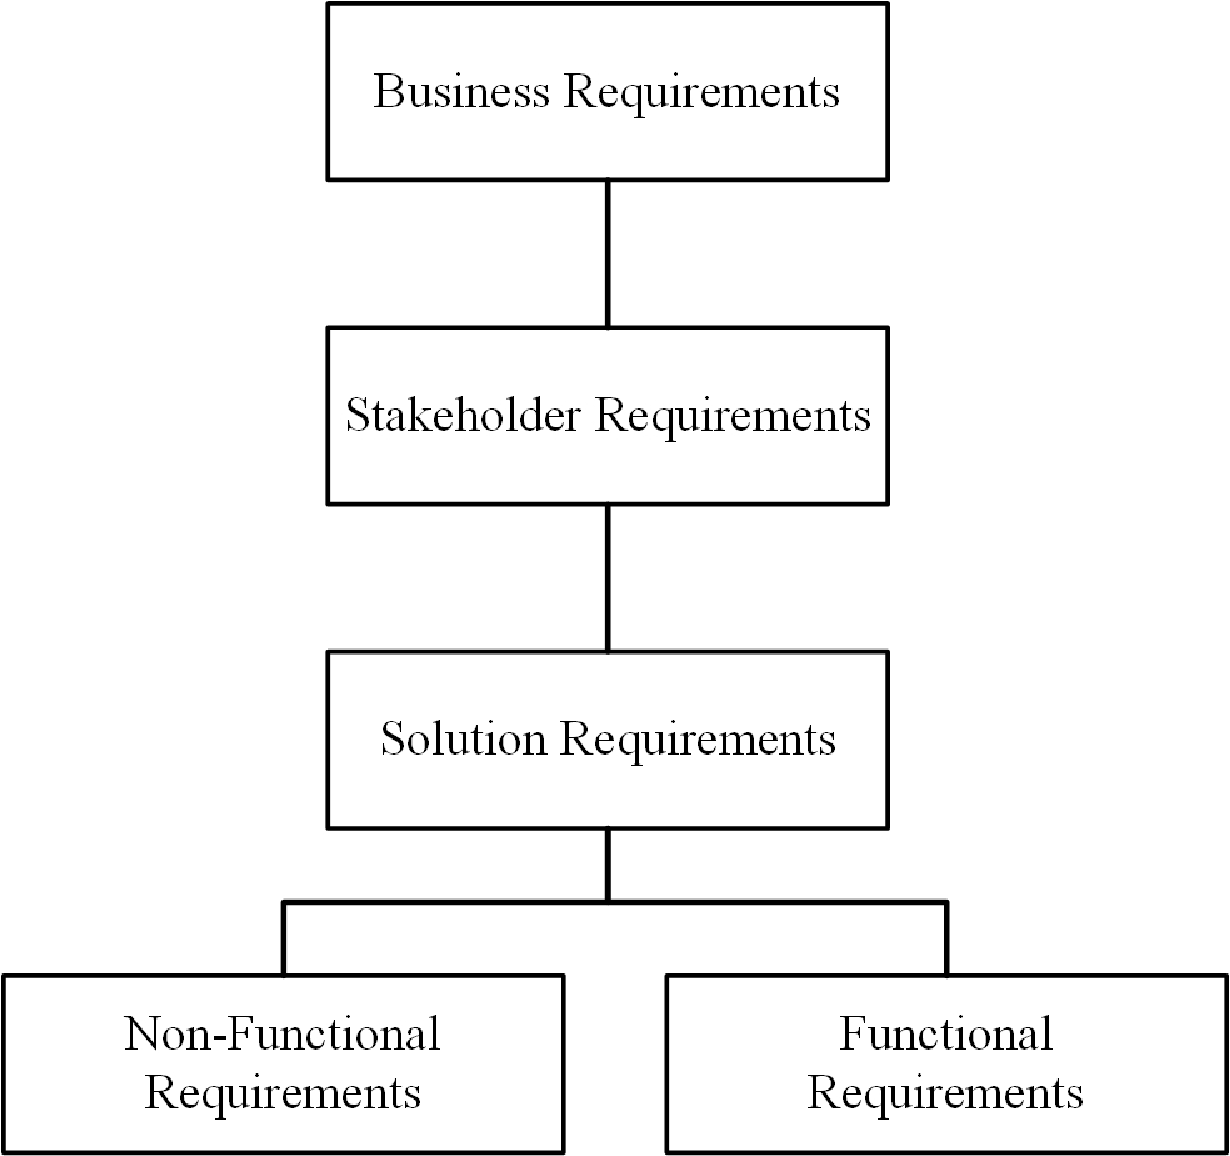
\includegraphics[width=0.45\textwidth]{images/business-requirements.pdf}
    \captionsetup{justification=centering}
    \caption[Workflow support for business needs]{Workflow support for business needs
                                                  (Wu and Buyya 2015 p. 66 fig. 2.12)}
    \label{fig:network-business}
\end{figure}

\subsection{Business Requirements}

The strategic analysis of a business can also be referred as a method that will allow the creation of the business
requirements, these requirements being the result of the analysis performed. As it can be seen in the figure 5,
the business requirements are the top level of the workflow support for the business needs and because of this
the business requirements must be developed as the analysis of business activities are performed.

\subsection{Stakeholder Requirements}

According to Wu and Buyya (2015) the stakeholder requirements depend largely on the stakeholder of the business
as the stakeholder represents all the persons involved in a technological project, while the stakeholder
requirements represent an interface that provides solutions between other stakeholders, the stakeholder
requirements will ensure that all other persons involved in a project as a group will be working towards
the same ultimate goal and because of this the requirements can be considered as a method of consolidation
or anticipation for the high-level business requirements that will allow the creation of comprehensive,
practical, measurable and realistic solution requirements.

\subsection{Solution Requirements}

The solution requirements of a specific business can be referred as the business requirements but in a more
comprehensive manner. They are constituted of two other sub sets of solution requirements; these two sub
sets are the non-functional and functional requirements which will be translated into project tasks
(Wu and Buyya 2015).

\section{Conclusions}

The background chapter has shown the importance of the maintenance actions that must be performed for computer
systems, technological systems and equipment in order to ensure the stability of the systems in cause. In this
chapter it was also discussed why businesses must take into account factors such as the labour investment and
costs which will increase due to inability of the business to understand that the classical reliability theory
related to computer systems or technological systems will not be able offer any solutions to the maintenance
or failure of systems problem which will ultimately lead to the consequences to be felt significantly by the
entities in cause if no measures are put in place to mitigate the failure events. In addition to the importance
of the maintenance events in this chapter it was discussed that the failure predictions must be accompanied
with a diagnostic of the failure root cause in order to be able to anticipate and execute the necessary actions
to allow the system to remain functional and in a stable state. After the root causes, faults and errors were
evaluated it was concluded that the hardware element presents a good candidate for further investigations in
order to accentuate the research towards this area which could lead to a decrease of 10\% of computer systems
failures in data centres, the failure events being represented by the hardware element. Further into the research
it was concluded that the maintenance solutions related to computer system or technological systems can be
categorised as either reactive maintenance solutions or predictive maintenance solutions, the latter one being
the focus of this research. During the extended research of the predictive maintenance solution it was concluded
that providing a solution to computer system failure predictions problem will present many challenges and
impediments due to the continuous increase of technological complexity and the dynamic runtime of computer
systems. After the hardware element was set as the centre of research for failure predictions, the hardware
elements that were investigated for possible failure predictions related to computer systems were the Central
Processing Unit (CPU), the Random-Access Memory (RAM) and the Hard-Disk Drive (HDD) component. It was concluded
that the Hard-Disk Drive it is more predispose to failure than the other components and it presents the best
candidate for failure predictions as it has the suitable attributes that will allow the failure predictions
happen. Once the predispose hardware component to failure has been identified, the software implications have
been investigated and it has been concluded that the certain applications will save relevant information into
system log files which could be beneficial to the process of failure predictions. The final evaluation was the
analysis of possible candidate machine learning algorithms that could solve the problem of technological systems
failure predictions, the Support Vector Machines (SVM) algorithm and the Hidden Markov Model (HMM) were evaluated
and both algorithms present promising results, the Hidden Markov Model having the best results with a precision
rate of 88.51\% in the favour of the Support Vector Machines with a 73\% accuracy. The machine learning algorithm
called Support Vector Machines (SVM) will be used for the implementation of the solution as this algorithm it is
used in association with the S.M.A.R.T indicators which are a core element for the failure predictions process.
\newline
\newline
Research Question: Is it possible to build a solution using the Support Vector Machines (SVM) algorithm for the
maintenance of computer systems problem?

